% Created 2019-08-27 Tue 12:58
% Intended LaTeX compiler: pdflatex
\documentclass[11pt]{article}
\usepackage[utf8]{inputenc}
\usepackage{lmodern}
\usepackage[T1]{fontenc}
\usepackage{fixltx2e}
\usepackage{graphicx}
\usepackage{longtable}
\usepackage{float}
\usepackage{wrapfig}
\usepackage{rotating}
\usepackage[normalem]{ulem}
\usepackage{amsmath}
\usepackage{textcomp}
\usepackage{marvosym}
\usepackage{wasysym}
\usepackage{amssymb}
\usepackage{amsmath}
\usepackage[theorems, skins]{tcolorbox}
\usepackage[version=3]{mhchem}
\usepackage[numbers,super,sort&compress]{natbib}
\usepackage{natmove}
\usepackage{url}
\usepackage{minted}
\usepackage{underscore}
\usepackage[linktocpage,pdfstartview=FitH,colorlinks,
linkcolor=blue,anchorcolor=blue,
citecolor=blue,filecolor=blue,menucolor=blue,urlcolor=blue]{hyperref}
\usepackage{attachfile}
\usepackage{geometry}
\geometry{margin=1.0in}
\usepackage{outline}
\usepackage{amsmath}
\usepackage{graphicx}
\usepackage{epstopdf}
\usepackage{siunitx}
\usepackage{fancyhdr}
\usepackage{hyperref}
\usepackage[labelfont=bf]{caption}
\setlength{\headheight}{15.2pt}
\def\dbar{{\mathchar'26\mkern-12mu d}}
\pagestyle{fancy}
\fancyhf{}
\renewcommand{\headrulewidth}{0.5pt}
\renewcommand{\footrulewidth}{0.5pt}
\lfoot{\today}
\cfoot{\copyright\ 2019 W.\ F.\ Schneider}
\rfoot{\thepage}
\lhead{\em{Computational Chemistry}}
\rhead{ND CHE 30324}
\setcounter{secnumdepth}{3}
\author{William F. Schneider}
\date{\today}
\title{CHE 30324 Outline}
\begin{document}

\setcounter{tocdepth}{2}
\tableofcontents

\begin{OPTIONS}
\end{OPTIONS}
\section{Refresher on Quantum Mechanics}
\label{sec:org988166c}
\subsection{Why quantum mechanics?}
\label{sec:org4934f2d}
Want to describe ``mechanics'' (equations of motion) of atomic-scale things,
like electrons in atoms and molecules

Why? These ultimately determine the energy, the shape, and all the properties
of matter.

\[\lambda  = h/p = h/mv\]

\emph{de Broglie wavelength} (1924)
\begin{equation}
\lambda  = h/p = h/mv
\end{equation}
\begin{equation}
h  = 6.626 \times 10^{-34}~\text{J s (Planck's constant)}
\end{equation}

\begin{table}[htbp]
\caption{Car vs electron as a quantum particle}
\centering
\begin{tabular}{lll}
\hline
 & Car & Electron\\
\hline
mass \(m\) & 1000 kg & 9.1\texttimes{} 10\(^{\text{-31}}\) kg\\
velocity \(v\) & 100 km/hr & \(0.01 c\)\\
 & typical value on the highway & typical value in an atom\\
momentum \(p\) & \SI{2.8e-4}{kg.m/s} & 2.7 \texttimes{} 10\(^{\text{-24}}\) kg m/s\\
wavelength \(\lambda\) & 2.4 \texttimes{} 10\(^{\text{-38}}\) m & 2.4 \texttimes{} 10\(^{\text{-10}}\) m\\
 & too small to detect.  Classical! & Comparable to size of an atom.\\
 &  & \emph{Must} treat with QM!\\
\hline
\end{tabular}
\end{table}

How to describe wave properties of an electron?  Schr\"{o}dinger equation (1926)

\begin{center}
Kinetic energy + Potential energy = Total Energy
\end{center}

Expressed as differential equation (Single particle, non-relativistic):
\begin{equation}
-\frac{\hbar^2}{2m}\nabla^2 \Psi(\mathbf{r},t) + V(\mathbf{r},t)  \Psi(\mathbf{r},t) = -i \hbar \frac{\partial}{\partial t}  \Psi(\mathbf{r},t)
\end{equation}

If the potential \(V\) is time-invariant, can use separation of variables to
show that the steady-state, time-independent solutions are characterized by an
energy \(E\) and described by:
\begin{eqnarray}
-\frac{\hbar^2}{2m}\nabla^2 \psi(\mathbf{r}) + V(\mathbf{r})  \psi(\mathbf{r}) = E \psi(\mathbf{r}) \\
\Psi(\mathbf{r},t) = \psi(\mathbf{r})e^{-iEt/\hbar}
\end{eqnarray}

\subsection{Postulates of Non-relativistic quantum mechanics}
\label{sec:orgeade7e1}
See table
\begin{table}
\begin{center}
    \caption{\large{Postulates of Non-relativistic Quantum Mechanics}}
   \begin{description}
    \item[Postulate 1:] {{\bf The physical state of a system is completely described by
        its wavefunction $\Psi$.}  In general, $\Psi$ is a complex function of the spatial
      coordinates and time.  $\Psi$ is required to be:}
    \begin{outline}
      \item{Single-valued}
      \item {continuous and twice differentiable}
      \item {square-integrable ($\int \Psi^*\Psi d\tau$ is defined over all finite domains)}
      \item {For bound systems, $\Psi$ can always be normalized such that $\int \Psi^*\Psi d\tau=1$}
    \end{outline}

  \item[Postulate 2:]  To every physical observable quantity $M$ there corresponds a
    Hermitian operator $\hat{M}$.  {\bf The only observable values of $M$ are the
      eignevalues of $\hat{M}$.}
    \begin{center}
    \begin{tabular}[h]{ccc}
      \hline
{\bf Physical quantity} & {\bf Operator} & {\bf Expression} \\
\hline
Position $x,y,z$ & $\hat{x},\hat{y},\hat{z}$ & $x\cdot, y\cdot, z\cdot$ \\ \\
Linear momentum $p_x, \ldots$ & $\hat{p}_x,\ldots $ & $\displaystyle -i\hbar\frac{\partial}{\partial
  x},\ldots $\\
Angular momentum $l_x, \ldots$ & $\hat{p}_x,\ldots $ & $\displaystyle -i\hbar \left
  (y\frac{\partial}{\partial z}-z\frac{\partial}{\partial y}\right ), \ldots $ \\
Kinetic energy $T$ & $\hat{T}$ & $\displaystyle -\frac{\hbar^2}{2m}\nabla^2$ \\
Potential energy $V$ & $\hat{V}$ & $V({\bf r},t)$ \\
Total energy $E$ & $\hat{H}$ & $\displaystyle -\frac{\hbar^2}{2m}\nabla^2+V({\bf r},t)$\\ \\
\hline
    \end{tabular}
  \end{center}
    \item[Postulate 3:] {If a particular observable $M$ is measured many times on many
      identical systems is a state $\Psi$, the average resuts with be the expectation
      value of the operator $\hat{M}$:
      \begin{equation*}
        \langle M \rangle = \int \Psi^* (\hat{M}\Psi)d{\bf\tau}
      \end{equation*}}
    \item[Postulate 4:] {The energy-invariant states of a system are solutions of the equation
        \begin{eqnarray*}
          \hat{H}\Psi({\bf r},t) & = & i\hbar\frac{\partial}{\partial t}\Psi({\bf r},t) \\
          \hat{H} & = & \hat{T}+\hat{V}
        \end{eqnarray*}
      The time-independent, stationary states of the system are solutions to the equation
      \begin{equation*}
        \hat{H}\Psi({\bf r}) = E\Psi(\bf{r})
      \end{equation*}
}
    \item[Postulate 5:] (The {\bf uncertainty principle}.)  Operators that do not commute
      $(\hat{A}(\hat{B}\Psi)\neq\hat{B}(\hat{A}\Psi))$ are called /conjugate/.
      Conjugate observables cannot be determined simultaneously to arbitrary accuracy.
      For example, the standard deviation in the measured positions and momenta of
      particles all described by the same $\Psi$ must satisfy $\Delta x\Delta p_x \geq \hbar/2$.
    \end{description}
\end{center}
\end{table}

\subsection{Notes on constants and units}
\label{sec:org3326162}
Resource on physical constants: \url{http://physics.nist.gov/cuu/Constants/}
Resource for unit conversions: \url{http://www.digitaldutch.com/unitconverter/}

Unit converter available in Calc mode of Gnu emacs \textbf{highly recommended}

\begin{table}[htbp]
\caption{Atomic units common for quantum mechanical calculations (see \url{http://en.wikipedia.org/wiki/Atomic\_units})}
\centering
\begin{tabular}{llll}
\hline
 & Atomic unit & SI unit & Common unit\\
\hline
Charge & \(e = 1\) & \(1.6021 \times 10^{-19}\) C & \\
Length & \(a_0 = 1\) (bohr) & \(5.29177 \times 10^{-11}\) m & 0.529177 \AA{}\\
Mass & \(m_e = 1\) & \(9.10938 \times 10^{-31}\) kg & \\
Angular momentum & \(\hbar = 1\) & \(1.054 572 \times 10^{-34}\) J s & \\
Energy & \(E_h = 1\) (hartree) & \(4.359744 \times 10^{-18}\) J & 27.2114 eV\\
Electrostatic force & \(1/(4\pi\epsilon_0) = 1\) & \(8.987552 \times 10^9\) C\(^{-2}\) N m\^{}2 & \\
Boltzmann constant &  & \(1.38065 \times 10^{-23}\) J K\(^{-1}\) & 8.31447 J/mol K\\
\hline
\end{tabular}
\end{table}


\begin{center}
Energy units
1 eV = 1.60218\texttimes{} 10\(^{\text{-19}}\) J = 96.485 kJ/mol = 8065.5 cm\(^{\text{-1}}\) = 11064 K kB
\end{center}

\subsection{Example: Energy states of an electron in a box}
\label{sec:orgcca0cb3}
System defined by potential experienced by particle:

\(V(\mathbf{r}) = 0,\qquad 0 < x,y,z < L\)

\(V(\mathbf{r}) = \infty,\qquad x,y,z \leq 0,\ x,y,z \geq L\)

\begin{center}
\begin{center}
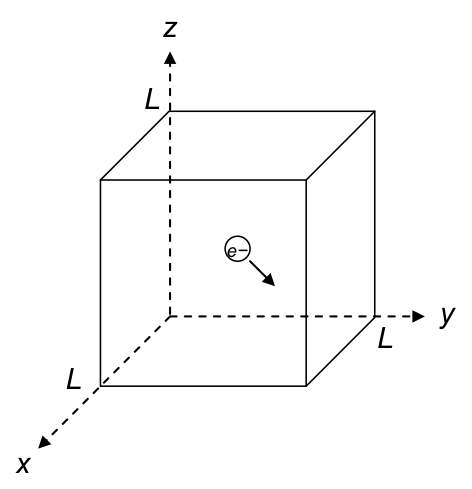
\includegraphics[width=0.3\textwidth]{./Images/Cube.png}
\end{center}
\end{center}

3D box \(\rightarrow\) 3 degrees of freedom/coordinates

\textbf{Schr\"{o}dinger equation}
\begin{equation}
-\frac{\hbar^2}{2m_e} \left ( \frac{\partial^2 }{\partial x^2} + \frac{\partial^2 }{\partial y^2} + \frac{\partial^2 }{\partial z^2} \right ) \psi(x,y,z) = E \psi(x,y,z)
\end{equation}
\begin{equation}
\psi(x,y,z) = 0, \quad x,y,z \leq 0,\ x,y,z \geq L
\end{equation}

A second-order, linear, partial differential equation.  Boundary value problem.
Solve by separation of variables.  Postulate \(\psi(x,y,z) = X(x)Y(y)Z(z)\).
Substituting and rearrange to get

\begin{equation}
-\frac{\hbar^2}{2m_e} \left (\frac{1}{X(x)}\frac{\partial^2 X(x)}{\partial x^2} + \frac{1}{Y(y)}\frac{\partial^2 Y(y)}{\partial y^2} + \frac{1}{Z(z)}\frac{\partial^2 Z(z)}{\partial z^2} \right ) = E \qquad 0 < x,y,z <L
\end{equation}

ftn x + ftn y + ftn z = constant \(\rightarrow\) each term must be constant.

\textbf{Equation for each dimension}
\begin{equation}
-\frac{\hbar^2}{2m_e}\frac{\partial^2 X(x)}{\partial x^2} = E_x X(x), \qquad X(0)=X(L) = 0
\end{equation}

Seek function that twice differentiated returns itself and satisfies
boundary conditions.
\begin{equation}
X(x) = \sin\frac{n_x\pi x}{L},\qquad n_x = 1,2,3,\ldots
\end{equation}

\begin{equation}
E_{n_x} = \frac{n_x^2\pi^2\hbar^2}{2 m_e L^2}
\end{equation}

Solutions called \emph{eigenfunctions} (or \emph{wavefunctions}) and \emph{eigenvalues}.  Characterized
by \emph{quantum numbers}, one for each degree of freedom.  These (and all QM) solutions have certain
special properties, including that they are orthonormal and form a complete set.

\textbf{Normalization}

Seek a constant such that the inner eigenfunction product is unity.
\begin{eqnarray}
C^2 \int_0^L \sin^2 \frac{n_x\pi x}{L} dx = C^2 L/2 = 1 \rightarrow C=\pm\sqrt{\frac{2}{L}}\\
X(x) = \pm\sqrt{\frac{2}{L}}\sin\frac{n_x\pi x}{L},\qquad n_x = 1,2,3,\ldots
\end{eqnarray}

\textbf{Orthonormal}
\begin{equation}
\langle X_{n_x} | X_{n^\prime_x} \rangle = \delta_{n_{x},n_x^\prime}\qquad
\text{Dirac notation}
\end{equation}

\begin{minted}[frame=lines,fontsize=\scriptsize,linenos]{python}
  import matplotlib, numpy
  matplotlib.use('Agg')
  import matplotlib.pyplot as plt
  fig=plt.figure(figsize=(4,2))
  x=numpy.linspace(-15,15)
  plt.plot(numpy.sin(x))
  fig.tight_layout()
  plt.savefig('images/python-matplot-fig.png')
  return 'images/python-matplot-fig.png' # return filename to org-mode
\end{minted}

\begin{center}
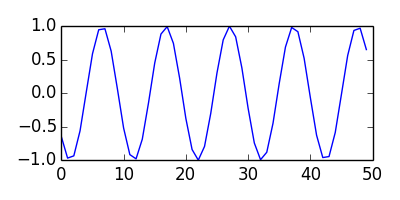
\includegraphics[width=.9\linewidth]{images/python-matplot-fig.png}
\end{center}


\begin{center}
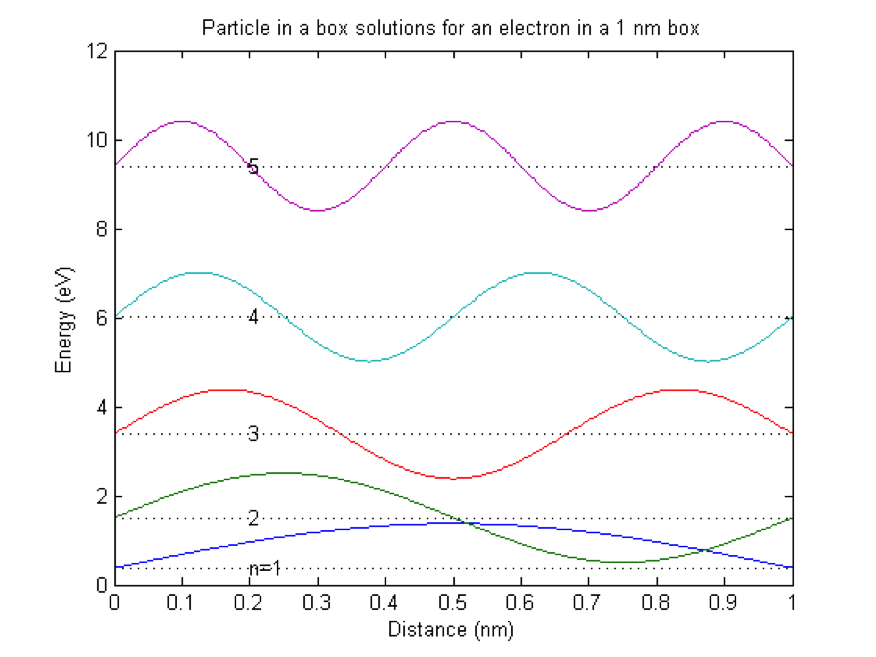
\includegraphics[width=0.75\textwidth]{./Images/SineWave.png}
\end{center}

\begin{itemize}
\item Energy increase with number of \emph{nodes}.

\item \(E\propto n^2, \Delta E \propto n, \Delta E/E \propto 1/n\).  \emph{Relative} spacing decreases with \(n\).

\item Is this real?  See \href{http://dx.doi.org/10.1021/jp053496l}{Ho, \emph{J. Phys. Chem. B} \textbf{2005}, \emph{109}, 20657}.
\end{itemize}

\textbf{Three-dimensional solutions}
\begin{equation}
\psi(x,y,z) = X(x)Y(y)Z(z) = \left ( \frac{2}{L} \right )^{3/2} \sin\frac{n_x\pi x}{L}\sin\frac{n_y\pi y}{L}\sin\frac{n_z\pi z}{L},\qquad n_{x},n_{y},n_{z}=1,2,3,\ldots
\end{equation}
\begin{equation}
\label{eq:2}
E = E_{x}+E_{y}+E_{z}=\frac{(n_{x}^{2}+n_{y}^{2}+n_{z}^{2}) \pi^{2}\hbar^{2}}{2 m L^{2}}
\end{equation}

\begin{center}
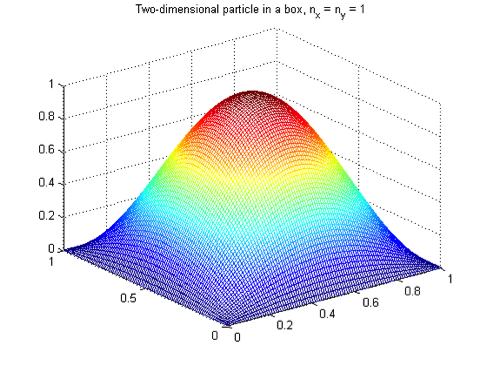
\includegraphics[width=0.5\textwidth]{./Images/2DSine1.png}
\end{center}
\begin{center}
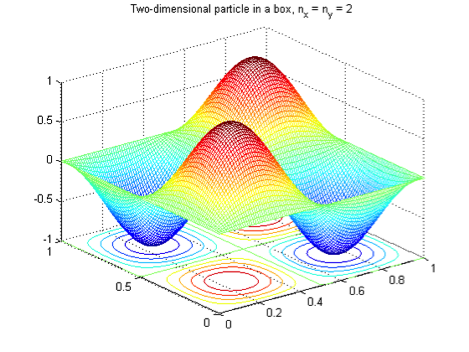
\includegraphics[width=0.5\textwidth]{./Images/2DSine2.png}
\end{center}


\begin{figure}[htbp]
\centering
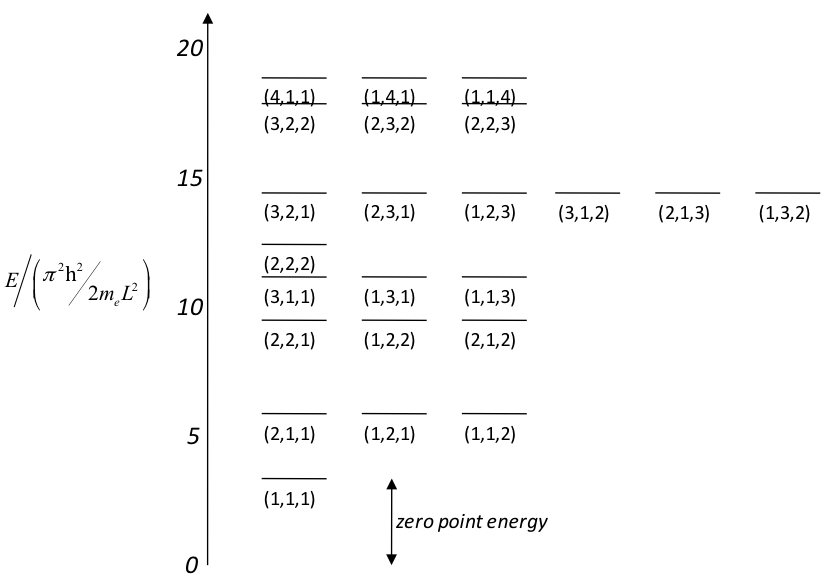
\includegraphics[width=.9\linewidth]{./Images/3DEnergyStates.png}
\caption{Energy sates of 3D Particle in a box}
\end{figure}

Properties of solutions:
\begin{itemize}
\item Symmetry of system introduces degeneracy in solutions
\item Energy depends on volume \(\rightarrow\) pressure!
\end{itemize}
\end{document}